\chapter{Lo Stage per ARPAV}
\label{2.0}
\thispagestyle{fancy} 

Il dipartimento di reti ed informatica deve affrontare la difficile sfida di mantenere la parità del bilancio, senza rinunciare alla qualità delle loro opere. Il responsabile del dipartimento, spinto da questa necessità, ha orientato la politica di scelta del personale, durante la fase di codifica, verso stagisti neo-laureati o laureandi. Questa scelta permette:

\begin{itemize}

	\item \textbf{maggior efficacia:} l'utilizzo di stagisti permette di ottimizzare le risorse di bilancio, diminuendo l'impatto sul \textit{budget};
	\item \textbf{maggiore efficacia:} menti fresche di studio e con bassa specializzazione permettono un'adesione a progetti nuovi ed innovativi con maggiore facilità rispetto a personale propenso a lavorare secondo processi prestabiliti.

\end{itemize}

\section{L'Esigenza di uno Stage}

Il dipartimento di reti ed informatica, al momento del mio inserimento, stava seguendo la progettazione e lo sviluppo di un pluviometro\ped{g} innovativo a basso costo da parte del \textit{FabLab}\ped{g} di Verona.
\begin{figure}[htbp]
\centering
\begin{minipage}[c]{.30\textwidth}
	\centering\setlength{\captionmargin}{0pt}%
	
\includegraphics[width=0.50\textwidth]{./capitoli/capitolo2/img/raspibo}
	\caption{Logo RaspiBO}
\end{minipage}%
\hspace{10mm}
\begin{minipage}[c]{.30\textwidth}
	\centering\setlength{\captionmargin}{0pt}%
	
\includegraphics[width=0.90\textwidth]{./capitoli/capitolo2/img/fablab}
	\caption{Logo FabLab}
\end{minipage}%
\end{figure} Questo incarico è stato proposto da parte di ARPAV per il progetto RE.S.M.I.A., il quale prevede il potenziamento dell'infrastruttura della rete di monitoraggio di ARPAV, tramite la progettazione di nuove stazioni meteorologiche. 
Contemporaneamente al progetto \textit{FabLab}, il responsabile del dipartimento stava seguendo il \textit{Gruppo Meteo} di \textit{RaspiBO}\ped{g} il quale sta sviluppando stazioni meteorologiche a basso costo, al momento sprovviste di pluviometro. La combinazione di questi due fattori ha creato la necessità di sviluppo di un sistema \textit{hardware} e \textit{software} che permettesse la gestione di un pluviometro tramite tecnologie a basso costo, ma con prestazioni adeguate alle richieste.



\section{Presentazione del Progetto}

La \textit{Small Project}, azienda italiana nata del 2004, appoggia il progetto \textit{Arduino} e ne è diventata il produttore principale. Arduino è una scheda elettronica di piccole dimensioni, con un microcontrollore e circuiteria di contorno per la realizzazione di progetti o prototipi. Il progetto Arduino, ormai avviato da qualche anno, ora conta svariate tipologie di schede con caratteristiche di prestazioni e prezzo differenti fra loro. Queste schede permettono una facile programmazione e una elastica implementazione a seconda delle necessità che il proprio lavoro richiedono. Per il progetto di \textit{stage}, è stato proposto l'utilizzo di una scheda \textit{Arduino UNO} (\url{www.arduino.cc/en/Main/ArduinoBoardUno}).

\begin{figure}[htbp]
\centering
\begin{minipage}[c]{.60\textwidth}
	\centering\setlength{\captionmargin}{0pt}
	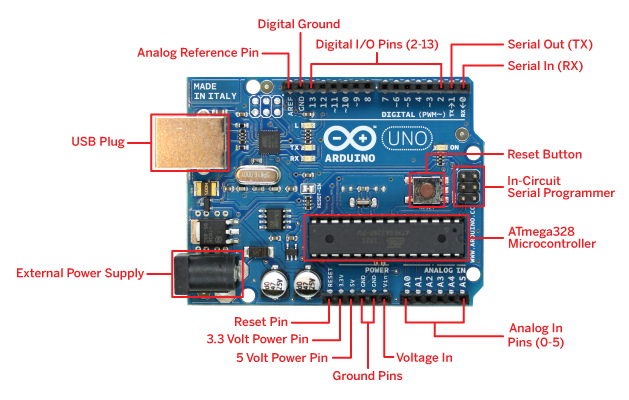
\includegraphics[scale=0.5]{./capitoli/capitolo2/img/ArduinoUNO}
	\caption{Scheda Arduino UNO}
\end{minipage}
\hspace{10mm}
\begin{minipage}[b]{.30\textwidth}
	\centering\setlength{\captionmargin}{0pt}%
	
\includegraphics[width=0.30\textwidth]{./capitoli/capitolo2/img/arduinologo}
	\caption{Logo Arduino}
\end{minipage}%

\end{figure}  

Il progetto prevede la progettazione e lo sviluppo di un dispositivo innovativo \textit{embedded} per la gestione di un pluviometro, lo studio per una gestione e memorizzazione efficiente di eventi di pioggia
mediante standardizzazione su protocollo MQTT\ped{g}, sviluppato su \textit{hardware} e \textit{firmware} ATMEL\ped{g}.

\begin{figure}[htbp]
	\centering
	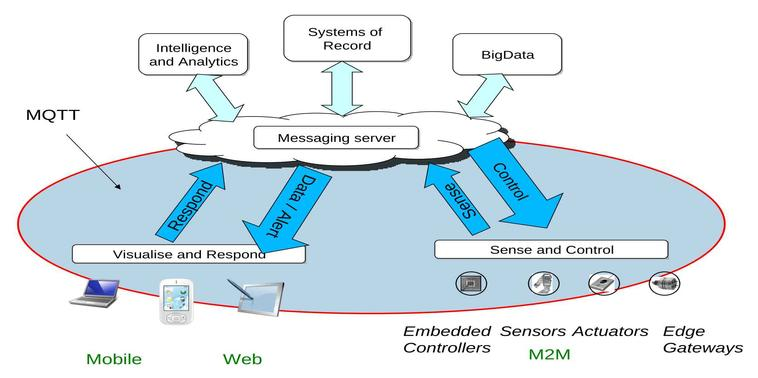
\includegraphics[scale=1]{./capitoli/capitolo2/img/mqtt}
	\caption{Esempio protocollo MQTT}

\end{figure}

Le componenti hardware saranno volutamente poco costose e quindi con limitate capacità di memorizzazione dati, pertanto sarà necessaria la ricerca di soluzioni che tengano in considerazione tale problematica. Nel progetto verrà richiesto l'utilizzo di due schede Arduino UNO, di cui una con lo scopo di gestione dei segnali ricevuti dall'\textit{hardware} del pluviometro, salvataggio e gestione dei dati, l'altra con la funzionalità di interrogazione della prima. Si sono riscontrate così due "tipologie" di schede:
\begin{itemize}
	\item \textbf{Scheda Slave:} scheda che si interfaccia direttamente con i segnali inviati dal pluviometro, che salva all'interno di una memoria i dati richiesti e li cancella in caso di necessità o richiesta;
	\item \textbf{Scheda Master:} scheda che permette l'interrogazione della \textit{scheda Slave}, tramite protocollo prestabilito e rimbalzi così i dati ricevuti all'utente che ne ha fatto richiesta.

\end{itemize}

La \textit{scheda Slave}, dovrà essere interamente progettata e realizzata all'interno del lavoro di \textit{stage}, per quanto riguarda la \textit{scheda master}, ciò che viene richiesto è la creazione di una libreria che permetta un facile accesso alle funzionalità di base richieste dal progetto e un'architettura tale che permetta facilmente integrazioni future.
Viene richiesto in oltre che tutto  progetto di \textit{stage} venga rilasciato tramite \textit{GNU GPL}\ped{g} su \textit{github}, provvisto di documentazione dei metodi e componenti \textit{software} associata per facilitare future modifiche o correzioni.


\subsection{Obiettivo dello Stage}

Gli obiettivi sono stati preposti durante i colloqui conoscitivi precedenti all'inizio dello \textit{stage}, evidenziando quelle che sarebbero state le caratteristiche salienti sufficienti per considerare soddisfacente il lavoro completo del tirocinio.

\begin{itemize}

	\item \textbf{Obiettivi esplorativi:} evidenziano il livello di capacità di indagine dello stagista nell'affrontare un ambiente nuovo in cui vengono utilizzate tecnologie mai affrontate durante il percorso accademico. Viene anche delineata l'attitudine ad analizzare i rischi legati all'utilizzo di componenti \textit{hardware} inesplorati da parte dell'agenzia e la capacità di risoluzioni dei problemi legati alle limitate prestazioni delle schede Arduino;
	
	\item \textbf{Obiettivi funzionali:} includono i requisiti minimi richiesti delle funzionalità per considerare il lavoro di \textit{stage} sufficiente alla propria conclusione. I requisiti descrivono le funzionalità che dovranno essere implementate nel progetto e rappresentano l'intento centrale di tutto il lavoro del tirocinio.
	
	\item \textbf{Obiettivi funzionali opzionali:} rappresentano l'insieme di requisiti che descrivono le funzionalità del progetto che non sono obbligatori per la completezza del lavoro di tirocinio, ma che rappresentano un valore aggiunto e desiderato da parte dei proponenti.
\end{itemize}

\subsubsection{Obiettivi Minimi Richiesti}
Di seguito vengono riportati gli obiettivi minimi che sono stati richiesti al momento di inizio \textit{stage}:

\begin{itemize}

	\item \textbf{Obiettivi esplorativi:}
	\begin{itemize}
	
		\item \textit{Acquisizione conoscenze elettronica di base:} dovendo affrontare un lavoro con schede \textit{hardware}, connettendo cavi, creando connessioni con dispositivi ausiliari e correnti elettriche, è strettamente necessario acquisire le conoscenze di base che permettano di lavorare in sicurezza e senza causare guasti alle strumentazioni;
		\item \textit{Comprensione ambiente Arduino:} il mondo Arduino offre una vasta scelta di modi in cui operare, dalla tipologia di linguaggio, agli strumenti di sviluppo. 
		\item \textit{Valutazione prestazione Arduino:} uno dei punti focali stabiliti ad inizio \textit{stage} è stato comprendere il prima possibile se la scheda fornita fosse sufficientemente adeguata per le richieste del progetto. Pur non essendo un vero e proprio obiettivo, mi è stato preposto come tale a causa della sua importanza, poiché la ricerca di un nuovo componente, o anche la sola acquisizione \textit{online}, avrebbe provocato considerevoli ritardi.
	
	\end{itemize}
	\item \textbf{Obiettivi funzionali:}
		\begin{itemize}
			\item \textit{Progettazione e sviluppo scheda Slave:} punto focale del lavoro di \textit{stage} è lo sviluppo della scheda connessa al pluviometro, che dovrà:
			\begin{itemize}
				\item Riconoscere gli impulsi inviati dal prototipo di pluviometro;
				\item Riconoscere segnali falsi positivi e non registrare dati infondati;
				\item Immagazzinare in una memoria i \textit{timestamp};
				\item Ottimizzare la gestione della memoria;
				\item Comunicare tramite \textit{protocollo I2C}\ped{g} con le componenti a lei connesse;
				\item Comunicare tramite protocollo I2C con la componente Master a due vie;
				\item Ritorno dei dati memorizzati;
				\item Cancellazione dei dati;
				\item Tenere traccia di eventuali \textit{overflow} dovuti alle basse prestazioni di memoria;
				\item Progettazione elastica che permetta l'inserimento futuro di nuovi protocolli di comunicazione o inserimento di nuovi componenti hardware;

			\end{itemize}
			\item \textit{Progettazione e sviluppo libreria Master:} secondo punto focale del progetto, sviluppo di una libreria che possa essere inserita in un contesto dove è già esistente una scheda Master a cui viene connesso il pluviometro con scheda Arduino integrata con il sistema Slave:
			\begin{itemize}
				\item Comunicazione tramite protocollo I2C con la scheda Slave del pluviometro;
				\item Progettazione elastica che permetta l'inserimento futuro di nuovi protocolli per la comunicazione con la scheda Slave;
				\item Richiesta per la ricezione dei dati inseriti in memoria della scheda Slave;
				\item Richiesta per la ricezione dei dati ancora non letti;
				\item Richiesta per la cancellazione dei dati già letti;
				\item Richiesta per la cancellazione dell'intera memoria della scheda Slave;
			\end{itemize}
		\end{itemize}

\end{itemize}



\subsubsection{Obiettivi Massimi Raggiungibili}

Di seguito vengono riportati gli obiettivi preposti ad inizio \textit{stage}, che non sono vincolanti alla conclusione dello stesso:
\begin{itemize}
		\item \textbf{Obiettivi esplorativi:} 
		\begin{itemize}
			\item \textit{Acquisizione conoscenze elettronica semi-avanzate:} imparare a formare uno schema elettronico di una scheda in modo da realizzare una componente \textit{hardware} nuova partendo da componenti separate e l'utilizzo di strumenti che ne permettano l'assemblo.
		\end{itemize}

		\item \textbf{Obiettivi funzionali opzionali:}
		\begin{itemize}
			\item \textit{Implementazione del codice su scheda Arietta\ped{g} :} adattamento, implementazione e test del codice precedentemente approvato su Arduino UNO in una scheda Arietta;
			\item \textit{Interfaccia di configurazione e ricezioni dati web o desktop:} progettazione e realizzazione di un \textit{tool web} o \textit{desktop} per la relazione diretta \textit{computer/web}-scheda Master;
			\item \textit{Comunicazione 3G con scheda Master:} implementazione di un dispositivo per la comunicazione via 3G tra dispositivo \textit{mobile} e la scheda Master;
		\end{itemize}

\end{itemize}
\subsection{Finalità del Progetto}
\begin{figure}[htbp]
\centering
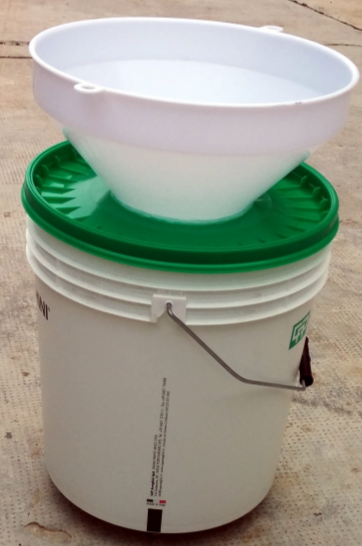
\includegraphics[scale=.3]{./capitoli/capitolo2/img/pluviometro}
\caption{Prototipo pluviometro FabLab}
\end{figure}

Nella realtà ARPAV il suddetto lavoro di \textit{stage}, oltre ad integrare una parte mancante del progetto RE.S.M.I.A., trova largo margine di prospettive future. Il progetto verrà rilasciato con licenza di utilizzo GNU GPL, quindi liberamente utilizzabile da chiunque. FabLab di Verona ha già lanciato un progetto parallelo successivo al lavoro di \textit{stage}: \textit{Tutti misurano, OpenPluvio}. Il progetto riprende il lavoro portato a termine e lo continua per introdurre un sistema di misurazione ambientale casalingo, amatoriale, che possa inviare i dati delle misurazioni effettuate a \textit{serve} dedicati. Lo scopo è facilitare il possesso di strumentazione di controllo ambientale a basso costo e la creazione una nuova rete di monitoraggio che possa integrare o arricchire i dati delle reti ufficiali.



\section{Vincoli di Progetto}

In questa sezione verranno descritti i vincoli del progetto che sono stati stabiliti ad inizio \textit{stage}, catalogati nel seguente modo:
\begin{itemize}
\item \textbf{Vincoli di dominio:} descrivono i vincoli di funzionalità, affidabilità e manutenibilità;
\item \textbf{Vincoli tecnologici:} descrivono gli strumenti di lavoro e le tecnologie obbligatorie;
\item \textbf{Vincoli metodologici:} descrivono le metodologie che imposte durante fase di \textit{stage};
\item \textbf{Vincoli temporali:} descrivono tappe obbligatorie da seguire durante l'attività lavorativa;
\end{itemize}

\subsection{Vincoli di Dominio}

Il sistema da realizzare dovrà immagazzinare una discreta quantità di dati in uno spazio di memoria ristretto. La necessità di sviluppare un algoritmo di compressione dei dati sarà estremamente necessario. I dati che dovranno essere immagazzinati vengono definiti \textit{timestamp}. I \textit{timestamp} sono un \textit{metadato} composto da più elementi:
\begin{itemize}
	\item \textbf{Data:} nel formato gg / mm / aaaa (esempio  12 05 2014);
	\item \textbf{Ora:} nel formato hh / mm / ss (esempio 12 02 35);
	\item \textbf{Contatore:} un numero che deve identificare il numero di \textit{timestamp} dall'ultima lettura effettuata.	
\end{itemize}

Ogni \textit{timestamp} verrà salvato in memoria successivamente all'interruzione di una basculata da parte del pluviometro. Una basculata avviene quando la vaschetta della bascula viene riempita fino ad un livello tale che il peso dell'acqua fa cadere la vaschetta. A seconda della tipologia di bascula il segnale può essere inviato diversamente. 

\begin{figure}[htpb]
\centering
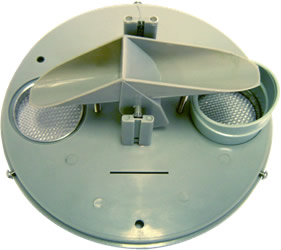
\includegraphics[scale=.4]{./capitoli/capitolo2/img/bascula}
\caption{Bascula di un pluviometro}

\end{figure}


Durante il lavoro di \textit{stage} verrà usato un pluviometro ancora sperimentale, quindi lo strumento di misurazione della bascula potrebbe risultare instabile e produrre dei segnali falsi positivi, con il risultato di immagazzinare erroneamente dei \textit{timestamp}. Uno dei vincoli principali del sistema dovrà essere l'affidabilità dei dati, i quali dovranno essere affidabili al 100\%. 

Il codice prodotto verrà rilasciato con licenza d'uso GPL, questo richiede che il codice sia chiaro e mantenibile. Per questo motivo è richiesta la presenza di documentazione che descriva le componenti \textit{software} e i metodi che contengono.

\subsection{Vincoli Tecnologici}

In questa sezione vengono riportate le tecnologie richieste per il completamento del lavoro stagistico.
\begin{itemize}

	\item \textbf{Arduino IDE:} \\
	\begin{figure}[htbp]
	\centering
	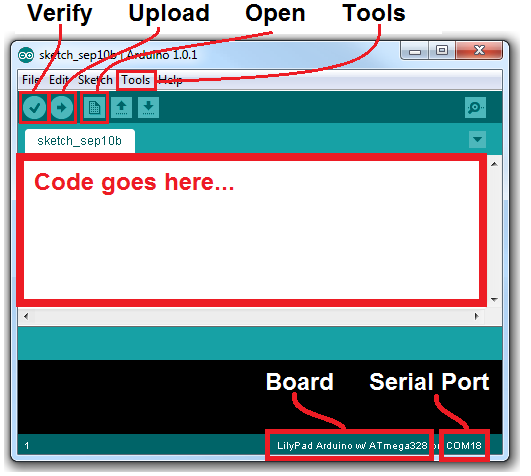
\includegraphics[scale=.4]{./capitoli/capitolo2/img/ide}
	\caption{Esempio di IDE Arduino}
	\end{figure}
	\textit{Arduino IDE} è un semplice \textit{framework} di programmazione multi-piattaforma che permette di caricare nella scheda Arduino il codice sorgente che si vuole implementare. E' il \textit{software }ufficiale fornito da Arduino e permette un utilizzo semplice della piattaforma. L'interfaccia dell'IDE permette di lavorare su di uno \textit{sketch} nel quale si deve caricare tutto il codice che si intende implementare nella \textit{board}. Sono obbligatorie le dichiarazioni di due metodi fondamentali:
	\begin{itemize}
		\item \textbf{void setup()} : metodo che viene evocato ogni volta che la scheda viene riavviata, all'interno del quale devono essere dichiarate le modalità di utilizzo dei \textit{pin} connessi alla scheda;
		\item \textbf{void loop()} : metodo che viene ripetuto continuamente dalla scheda in un \textit{loop} infinito, finché viene mantenuta energia o non viene effettuato il \textit{reset}. 	
	
	\end{itemize}
	La sua semplicità rende questo strumento anche altrettanto limitato nella flessibilità di utilizzo. Per organizzare il codice in maniera strutturata per classi è necessario l'utilizzo di uno strumento secondario. L'IDE Arduino infatti permette la compilazione e l'\textit{upload} del codice presente solo nello \textit{sketch}. Senza l'utilizzo di un \textit{framework} esterno, bisognerebbe dichiarare tutte le classi all'interno di un unico \textit{file}.
	
	
	\item \textbf{Arduino UNO}:\\
	Come descritto in precedenza mi è stato richiesto l'utilizzo di una scheda Aduino UNO. Le specifiche tecniche di questa \textit{board} sono:
	\begin{itemize}
	\item \textit{Microcontroller}:	ATmega328;
	\item \textit{Operating Voltage}:	5V;
	\item \textit{Input Voltage (recommended)}: 7-12V;
	\item \textit{Input Voltage (limits)}:	6-20V;
	\item \textit{Digital I/O Pins	}: 14 (of which 6 provide PWM output);
	\item \textit{Analog Input Pins}: 6;
	\item \textit{DC Current per I/O Pin}:	40 mA;
	\item \textit{DC Current for 3.3V Pin}:	50 mA;
	\item \textit{SRAM}:	2 KB (ATmega328);
	\item \textit{EEPROM}:	512 Byte (ATmega328);
	\item \textit{Clock Speed}:	16 MHz;
	\item \textit{Length}:	68.6 mm;
	\item \textit{Width}:	53.4 mm;
	\item \textit{Weight}: 	25 g.
	\end{itemize}

	La scelta di questa scheda sono ricadute per i seguenti motivi:
	\begin{itemize}
	
	\item \textit{Affidabilità:} il prodotto 100\% italiano ha alle spalle una lunga storia di successi che hanno reso questo prodotto famoso per la sua affidabilità e robustezza;
	\item \textit{Feedback utenti:} poiché il prodotto è in commercio da qualche anno, i numerosi utenti che ne hanno fatto utilizzo hanno creato una solida rete di \textit{feedback} e risoluzione dei problemi;
	\item \textit{Riutilizzo software:} queste schede sono già state ampiamente usate per uno svariato numero di progetti con licenza gratuita, questo comporta la facile reperibilità \textit{online} di codice utile;
	\item  \textit{Componenti esterne:} molti produttori di componenti \textit{hardware} esterni, come sensori o schede di interfacce, forniscono librerie di interfacce perfettamente funzionanti e testati con l'ambiente Arduino;
	\item \textit{Prezzo:} 	
	il prezzo di una scheda Arduino si aggira sui 20 euro, mentre il microcontrollore ATmega328 dai 3 ai 5 euro. Se si utilizzassero solamente schede di questo tipo per il progetto, il risultato finale non risulterebbe economico. Durante la fase di codifica verranno usate due schede Arduino UNO per velocizzarne lo sviluppo, invece, il prodotto finale sarà composto da \textit{board} personalizzata che utilizzerà un microcontrollori con il codice già caricato, compatta ed economica.
	
	\end{itemize}


\item \textbf{Tiny-RTC (Real Time Clock Module)}\\
Componente \textit{hardware} per la misurazione del tempo. \textit{Tiny-RTC} non è altro che un modulo \textit{hardware} con la funzionalità di orologio configurabile tramite \textit{sketch} Arduino e provvisto di protocolli di I2C per l'interrogazione del modulo per il ritorno di data ed ora. 
\begin{figure}[htbp]
\centering
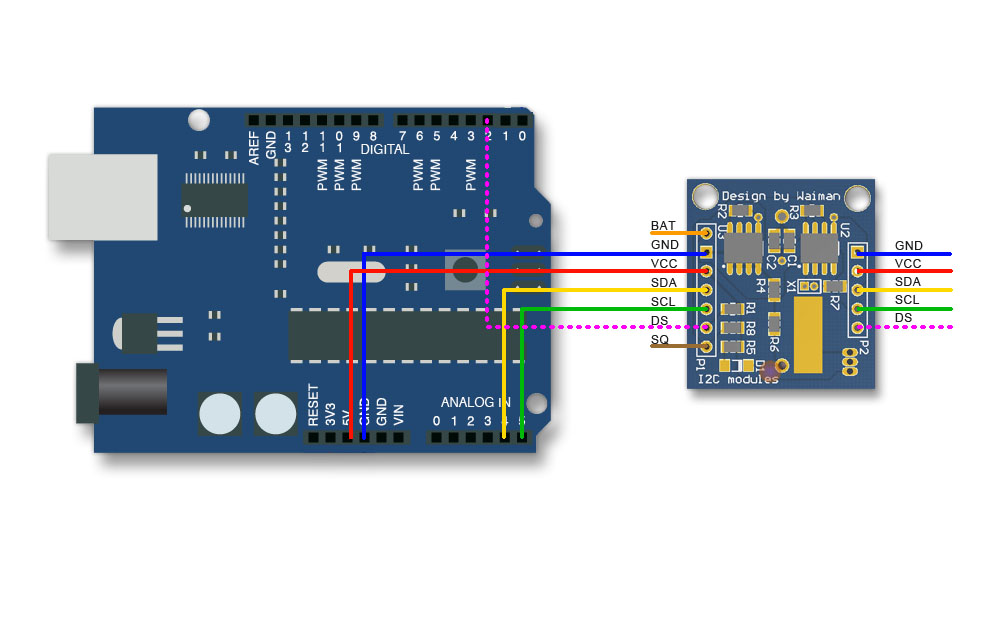
\includegraphics[scale=.3]{./capitoli/capitolo2/img/rtc}
\caption{Tiny RTC connessa a scheda Arduino UNO}

\end{figure}
 
Il modulo deve essere connesso alla \textit{board} Arduino tramite \textit{bus I2C} come mostrato nella figura 2.8. \\

Specifiche tecniche:
\begin{itemize}
    \item 3.0-5.5V input voltage
    \item Waterproof
    \item -55°C to+125°C temperature range
    \item ±0.5°C accuracy from -10°C to +85°C
    \item 1 Wire interface


\end{itemize}



Descrizione delle connessioni:

\begin{itemize}
\item \textbf{BAT}: 	Battery voltage 	
\item \textbf{GND}:	Ground 	Ground
\item \textbf{VCC}: Power the module and charge the battery
\item \textbf{SDA}: 	I2C data for the RTC
\item \textbf{SCL}:   I2C clock for the RTC
\item \textbf{DS}: 	Sensor output 	
\item \textbf{SQ}: 	Square wave output 
\end{itemize}
	
	
\item \textbf{Qt Creator}\\
\begin{figure}[htbp]
\centering

\includegraphics[scale=.8]{./capitoli/capitolo2/img/qt}
\caption{Logo Qt}
\end{figure}
Non mi è stato propriamente imposto l'utilizzo di \textit{Qt-Creator}, ma dal momento che mi era stato vivamente consigliato e durante il mio iter universitario ho avuto occasione di utilizzarlo frequentemente, è stato concordato sin dall'inizio il suo utilizzo per la codifica del codice.
\end{itemize}

\subsection{Vincoli Metodologici}

Come metodologie di lavoro mi sono state lasciate molte libertà, fatta eccezione per:

\begin{itemize}
	\item \textbf{Sistema di controllo di versionamento}\\
		\begin{figure}[htbp]
\centering
\begin{minipage}[c]{.45\textwidth}
	\centering\setlength{\captionmargin}{0pt}
	
\includegraphics[width=0.50\textwidth]{./capitoli/capitolo2/img/github}
	\caption{Logo GitHub}
\end{minipage}
\hspace{10mm}
\begin{minipage}[c]{.45\textwidth}
	\centering\setlength{\captionmargin}{0pt}%
	
\includegraphics[width=0.50\textwidth]{./capitoli/capitolo2/img/bitbucket}
	\caption{Logo Bitbucket}
\end{minipage}%

\end{figure}  
 Il responsabile del dipartimento mi ha richiesto l'utilizzo di \textit{git hub} come \textit{repository} del mio codice per la parte riguardante ARPAV. Invece il responsabile di FabLab ha richiesto l'utilizzo di un \textit{repository} di \textit{bit-bucket} privato per il codice da utilizzare durante il periodo di \textit{testing} dei dispositivi assieme al prototipo pluviometro.

\item \textbf{Rilascio continuo di prototipi}\\
	FabLab di Verona ha contemporaneamente molti progetti in corso d'opera, di cui buona parte assegnati sempre dal dipartimento di reti ed informatica di Padova. Con l'inizio del mio lavoro, l'officina ha dovuto spostare maggiormente il baricentro dell'attenzione sul progetto pluviometro. Per questo motivo mi è stato richiesto di organizzare il mio lavoro con modalità di progettazione e sviluppo attraverso \textit{prototipi}. 
	
\item \textbf{Relazioni avanzamento lavoro}\\
	Alla fine di ogni settimana ero tenuto ad aggiornare FabLab dei progressi ottenuti tramite una breve relazione da inviare via \textit{mail} direttamente al responsabile dell'officina.
\end{itemize}


\subsection{Vincoli Temporali}

L'Università di Padova rende obbligatorio lo svolgimento del lavoro di \textit{stage} nell'arco di 300 - 320 ore. Durante i colloqui conoscitivi è stato redatto un documento  di pianificazione del lavoro dove si sancivano le ore di lavoro effettive e come queste saranno suddivise. Il lavoro di \textit{stage} è stato dunque stabilito doversi svolgere in 320 nell'arco di 9 settimane. Un vincolo esterno importante da considerare è stata la necessità di avere sufficiente codice da avere un prototipo funzionante prima delle vacanze di Natale, da consegnare a \textit{FabLab} di Verona per poter iniziare i primi \textit{test} sul prototipo di pluviometro. 


